The general second degree equation can be expressed as follows,
\begin{align}
\vec{x^T}\vec{V}\vec{x}+2\vec{u^T}\vec{x}+f=0\label{eq:solutions/40/3/eqmain}
\end{align}
From the given second degree equation we get,
\begin{align}
\vec{V} &= \myvec{3&-\sqrt{3}\\-\sqrt{3}&1}\\ \label{eq:solutions/40/3/given1}
\vec{u} &= \myvec{3\\-2}\\ 
f &= 5 \label{eq:solutions/40/3/given2}
\end{align}
Expanding the determinant of $\vec{V}$ we observe, 
\begin{align}
\mydet{3&-\sqrt{3}\\-\sqrt{3}&1} = 0 \label{eq:solutions/40/3/eq2.1}
\end{align}
Also
\begin{align}
    \mydet{\vec{V}&\vec{u} \\\vec{u}^T & f}=
    \mydet{3&-\sqrt{3}&3\\-\sqrt{3}&1 &-2\\3 &-2&5}
    \neq 0\label{eq:solutions/40/3/eq2.2}\end{align}
Hence from \eqref{eq:solutions/40/3/eq2.1} and \eqref{eq:solutions/40/3/eq2.2} we conclude that given equation is a parabola. The characteristic equation of $\vec{V}$ is given as follows,
\begin{align}
\mydet{\vec{V}-\lambda\vec{I}} = \mydet{3-\lambda &-\sqrt{3}\\-\sqrt{3}& 1-\lambda} &= 0\\
\implies \lambda^2-4\lambda &= 0\label{eq:solutions/40/3/eqchar}
\end{align}
Hence the characteristic equation of $\vec{V}$ is given by \eqref{eq:solutions/40/3/eqchar}. The roots of \eqref{eq:solutions/40/3/eqchar} i.e the eigenvalues are given by
\begin{align}
\lambda_1=0, \lambda_2=4\label{eq:solutions/40/3/eqeigenvals}    
\end{align}
The eigen vector $\vec{p}$ is defined as, 
\begin{align}
\vec{V}\vec{p} &= \lambda\vec{p}\\
\implies\brak{\vec{V}-\lambda\vec{I}}\vec{p}&=0 \label{eq:solutions/40/3/eqev}
\end{align}
for $\lambda_1=0$,
\begin{align}
\brak{\vec{V}-\lambda_1\vec{I}}&=\myvec{3&-\sqrt{3}\\-\sqrt{3}&1}\xleftrightarrow[R_1=\frac{1}{\sqrt{3}}R_1]{R_2=R_1+R_2}\myvec{\sqrt{3}&-1\\0&0}\label{eq:solutions/40/3/eq2.3.0}
\end{align}
Substiuting equation \ref{eq:solutions/40/3/eq2.3.0} in equation \ref{eq:solutions/40/3/eqev} and upon normalizing we get we get
\begin{align}
\implies\vec{p_1}&=\myvec{1/2\\\sqrt{3}/2} \label{eq:solutions/40/3/eq2.3}
\end{align}
Again, for $\lambda_2=4$,
\begin{align}
\brak{\vec{V}-\lambda_2\vec{I}}&=\myvec{-1&-\sqrt{3}\\-\sqrt{3}&-3}\xleftrightarrow[R_1=-\sqrt{3}R_1]{R_2=-\sqrt{3}R_1+R_2}\myvec{1&\sqrt{3}\\0&0} \label{eq:solutions/40/3/eq2.3.1}
\end{align}
Substiuting equation \ref{eq:solutions/40/3/eq2.3.1} in equation  \ref{eq:solutions/40/3/eqev} and upon normalizing we get
\begin{align}
        \vec{p_2}&=\myvec{-\sqrt{3}/2 \\1/2} \label{eq:solutions/40/3/eqp1}
\end{align}
The matrix $\vec{P}$,
\begin{align}
\vec{P}&=\myvec{\vec{p_1}&\vec{p_2}}=\myvec{1/2&-\sqrt{3}/2\\\sqrt{3}/2&1/2} \\
\vec{D}&=\myvec{0&0\\0&4}
\end{align}
\begin{align}
    \eta=2\vec{p_1}^T\vec{u}=3-2\sqrt{3} 
\end{align}
The focal length of the parabola is given by:
\begin{align}
    \abs{\frac{\eta}{\lambda_2}} 
    = \abs{\frac{3-2\sqrt{3}}{4}} = 0.116
\end{align}
When $\mydet{\vec{V}}=0$, \eqref{eq:solutions/40/3/eqmain} can be written as
\begin{align}
    \vec{y^T}\vec{D}\vec{y}&=-\eta\myvec{1&0}\vec{y}\label{eq:solutions/40/3/eq2.4}
    \intertext{And the vertex $\vec{c}$ is given by }
    \myvec{\vec{u^T}+\frac{\eta}{2}\vec{p_1^T} \\ \vec{V}}\vec{c}=
    \myvec{-f \\ \frac{\eta}{2}\vec{p_1}-\vec{u}}\label{eq:solutions/40/3/eqa} 
\end{align}
Substituting the found values
\begin{align}
\vec{u}^T + \frac{\eta}{2}\vec{p_1}^T = \myvec{3&-2}+\frac{3-2\sqrt{3}}{2}\myvec{\frac{1}{2}&\frac{\sqrt{3}}{2}}\\
\implies\vec{u}^T + \frac{\eta}{2}\vec{p_1}^T =\myvec{\frac{15-2\sqrt{3}}{4}&\frac{-14+3\sqrt{3}}{4}}\label{eq:solutions/40/3/eq2.23} \\
\frac{\eta}{2} \vec{p_1} -\vec{u}= \myvec{\frac{-9-2\sqrt{3}}{4}\\ \frac{2+3\sqrt{3}}{4}}\label{eq:solutions/40/3/eq2.24}
\end{align}
using equations \eqref{eq:solutions/40/3/given1},\eqref{eq:solutions/40/3/given2},\eqref{eq:solutions/40/3/eq2.3},\eqref{eq:solutions/40/3/eq2.23},\eqref{eq:solutions/40/3/eq2.24} and \eqref{eq:solutions/40/3/eq2.3} in \eqref{eq:solutions/40/3/eqa}
\begin{align}
    \myvec{\frac{15-2\sqrt{3}}{4}&\frac{-14+3\sqrt{3}}{4}\\3 & -\sqrt{3}\\ -\sqrt{3}& 1}\vec{c} =\myvec{ -5\\\frac{-9-2\sqrt{3}}{4}\\ \frac{2+3\sqrt{3}}{4}}\label{eq:solutions/40/3/eqcen}
\end{align}
By performing row reductions on augmented matrix
\begin{multline}
\myvec{\frac{15-2\sqrt{3}}{4}&\frac{-14+3\sqrt{3}}{4}&-5\\3 & -\sqrt{3}&\frac{(-9-2\sqrt{3})}{4}\\ -\sqrt{3}& 1&\frac{2+3\sqrt{3}}{4}}{R_2\xleftrightarrow[]{}{R_1}}\\
\myvec{3 & -\sqrt{3}&\frac{(-9-2\sqrt{3})}{4}\\\frac{15-2\sqrt{3}}{4}&\frac{-14+3\sqrt{3}}{4}&-5\\-\sqrt{3}& 1&\frac{2+3\sqrt{3}}{4} }
\end{multline}
\begin{multline}
\myvec{3 & -\sqrt{3}&\frac{(-9-2\sqrt{3})}{4}\\\frac{15-2\sqrt{3}}{4}&\frac{-14+3\sqrt{3}}{4}&-5\\-\sqrt{3}& 1&\frac{2+3\sqrt{3}}{4}}
\xleftrightarrow[]{R_2\leftarrow R_2-\frac{15-2\sqrt{3}}{12}R_1}\\
\myvec{3 & -\sqrt{3}&\frac{(-9-2\sqrt{3})}{4}\\0 & 2(\sqrt{3}-2) & \frac{(4\sqrt{3}-39)}{16}\\\sqrt{3}& 1&\frac{2+3\sqrt{3}}{4}}
\end{multline}
Therefore, 
\begin{multline}
 \myvec{3 & -\sqrt{3}&\frac{(-9-2\sqrt{3})}{4}\\0&2(\sqrt{3}-2)&\frac{(4\sqrt{3}-39)}{16}\\-\sqrt{3}& 1&\frac{(2+3\sqrt{3})}{4}}\xleftrightarrow[]{R_3\leftarrow R_3+\frac{1}{\sqrt{3}}R_1}\\
\myvec{3 & -\frac{433}{250}&-\frac{311}{100}\\0 & -\frac{107}{200} & -2\\0& 0&0}
\end{multline}
\begin{figure}[!h]
    \centering
    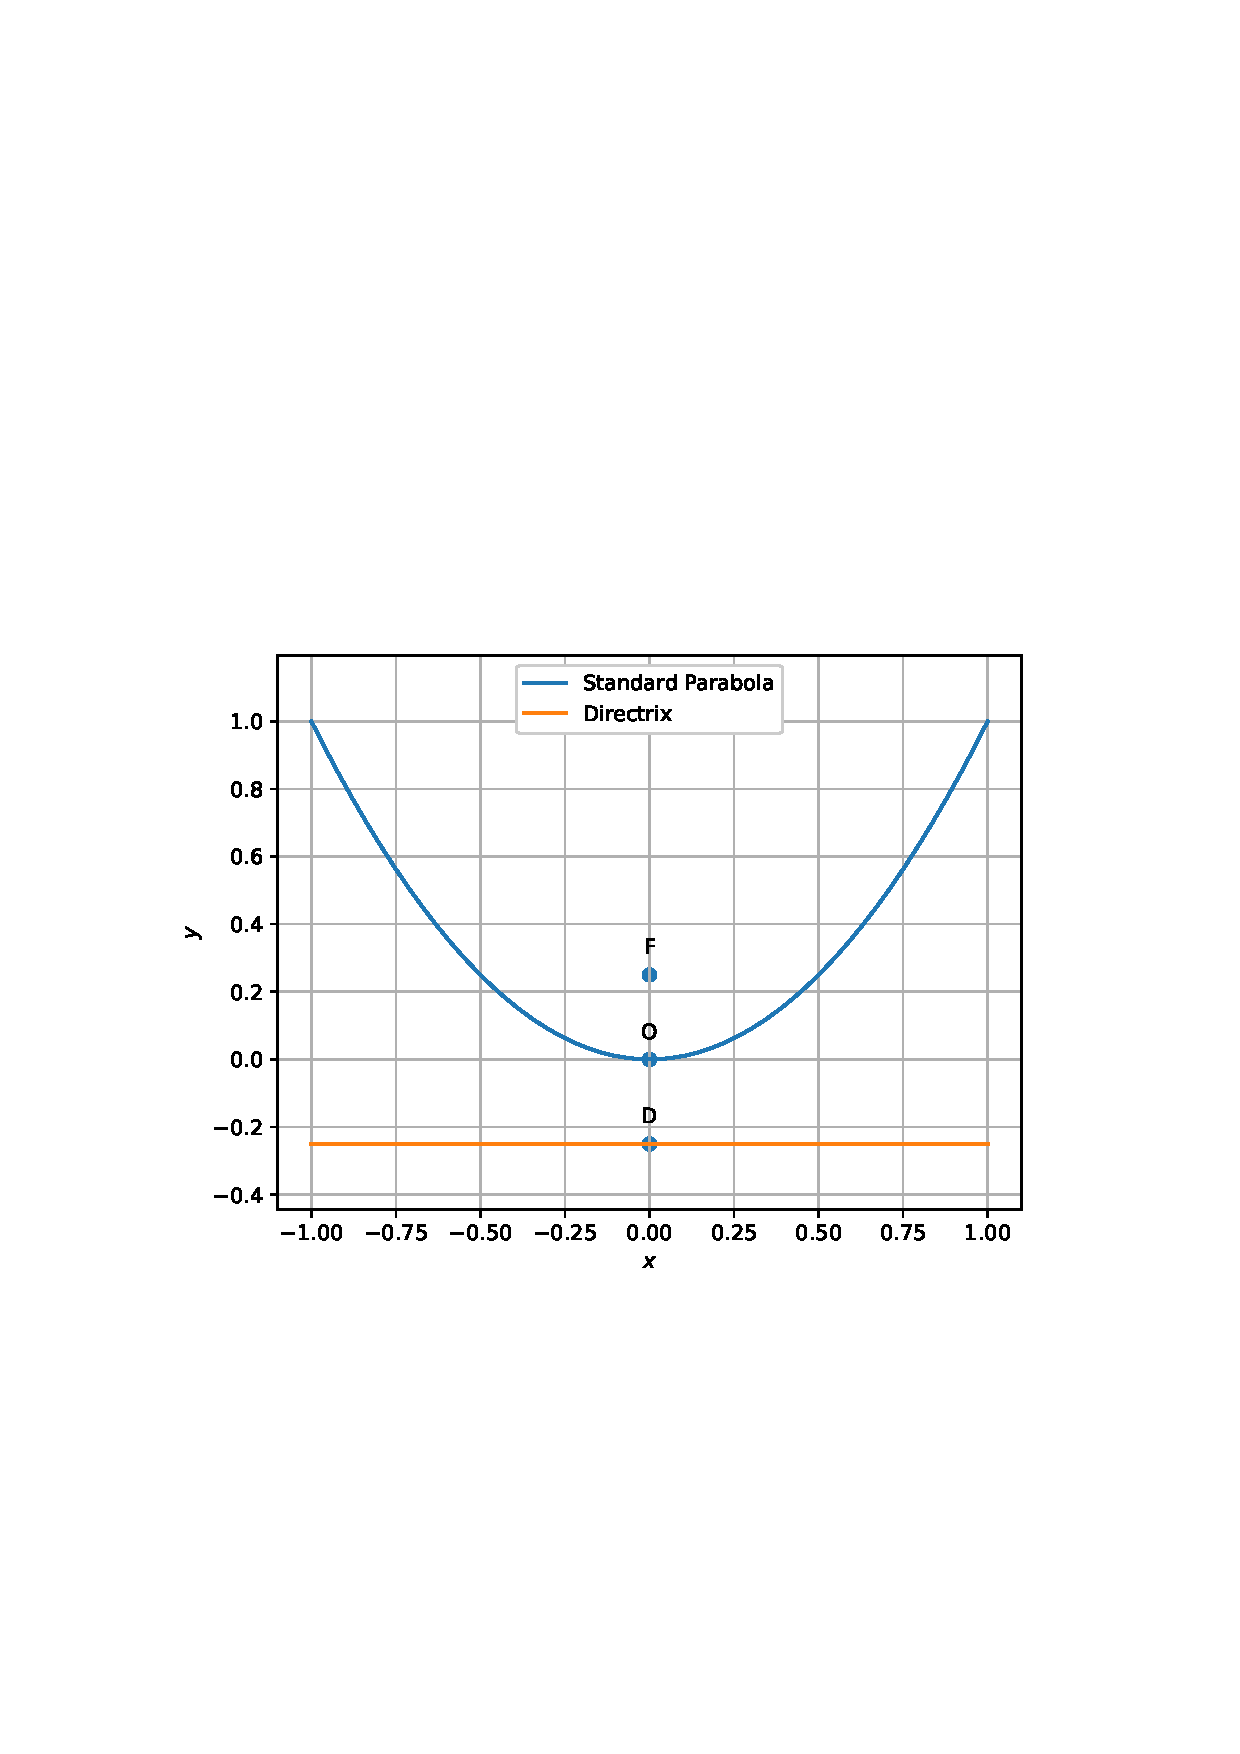
\includegraphics[width=\columnwidth]{./solutions/40/3/parabola.png}
    \caption{Parabola with the center c}
    \label{eq:solutions/40/3/Fig:1}
\end{figure}
\begin{multline}
\myvec{3 & -\frac{433}{250}&-\frac{311}{100}\\0 & -\frac{107}{200} & -2\\0& 0&0}\xleftrightarrow[]{R_1\leftarrow \frac{R_1}{{3}}}\\\myvec{1& -\frac{433}{750}&-\frac{311}{300}\\0 & -\frac{107}{200} & -2\\0& 0&0}
\end{multline}
\begin{multline}
\myvec{1 & -\frac{433}{750}&-\frac{311}{300}\\0 & -\frac{107}{200} & -2\\0& 0&0}\xleftrightarrow[]{R_2\leftarrow \frac{-200}{{107}}R_2}\\
\myvec{1 & -\frac{433}{750}&-\frac{311}{300}\\0 & 1 & \frac{400}{107}\\0& 0&0}
\end{multline}

\begin{multline}
\myvec{1 & -\frac{433}{750}&-\frac{311}{300}\\0 & 1 & \frac{400}{107}\\0& 0&0}\xleftrightarrow[]{R_1\leftarrow R_1+\frac{433}{{750}}R_2}\\
\myvec{1 & 0&\frac{12001}{10700}\\0 & 1 & \frac{400}{107}\\0& 0&0}\label{eq:solutions/40/3/eq7}
\end{multline}
On solving for values of $\vec{c}$ from \eqref{eq:solutions/40/3/eq7} 
 The vertex of parabola is $\vec{c}$=$\myvec{\frac{12001}{10700}\\\frac{400}{107}}$.
 
